\section{Making symbols for gschem}
Using \texttt{gschem} itself is one way to view and modify device attributes.  This section will describe how to use \texttt{gschem} to create and modify parts to be used in schematics. The attributes that must be present in my current scheme are: \texttt{refdes}, \texttt{device}, \texttt{value}, \texttt{description}, \texttt{footprint}, and \texttt{comment}.

\rednote{When you include a part in a schematic, \texttt{gschem} associates the part filename with the schematic.  Thus, changes made to the part files outside of the schematic will automatically update to the schematic.  This is bad when you ``translate'' the symbol when editing it, because the symbol will then move around on all the schematics it's associated with.}

\subsection{Making symbols for electrical and non-electrical parts}
Electrical symbols are those that have pins and make connections you can describe with a netlist.  Non-electrical symbols are for parts like nuts and bolts that should be included in the bill of materials but not the netlist.  Non-electrical parts need the \texttt{device}, \texttt{part}, \texttt{refdes}, and \texttt{value} attributes.

\subsubsection{Making a new symbol from scratch}

%Numbered directions for making gschem part
\begin{enumerate}
\item Run \texttt{gschem} -- bring up a blank schematic page.  Get rid of the default titleblock.
\item Draw the symbol
	\subitem Lines and pins should be drawn with 0.1 inch snap to grid.  Use  \textsl{Options} $\rightarrow$ \textsl{Snap grid spacing} to set grid size and be sure to turn snapping on.

\item (Electrical symbols) Add pins with \textsl{Add} $\rightarrow$ \textsl{pin}
	\subitem Pins should be 0.3 inches long and have their red ends pointing away from the symbol -- net connections are made at the red ends
	\subitem Pins should be at least 0.4 inches from their neighbors

\item (Electrical symbols) Add pin attributes: \texttt{pinnumber}, \texttt{pinseq}, \texttt{pinlabel}
	\subitem \texttt{pinseq} just tells gschem the order to output pins when it makes a netlist.
	\subitem The \texttt{pinnumber} attribute must match up with the ones you use for your footprints.  This will label pins on the netlist, so make this ``value only'' visible.  If you want the pin number to be visible, it should be positioned 50 mils away from its pin.
	\subitem The \texttt{pinlabel} attribute is just for information.  It lets you find the pin entry if you ever need to edit the raw text file for the symbol.


\item (Electrical symbols) Add the component's footprint attribute
    \subitem Make this attribute invisible, but edit the attribute (after turning the invisible text on) to select ``show name and value.''  Then both the attribute name and value will show up when you display invisible text.
    \subitem Example: \verb8footprint=2pin_MTA100_pol8
    
    \nailnote{Look in the project's eda\textbackslash footprints for available footprints.  The file footnotes.org may have some footprint-specific notes.  Use \texttt{\$pcb footprint.fp} to see a footprint.  See section \ref{footprint_section} beginning on page \pageref{footprint_section} for more information about footprints.}

\item Add the component's device attribute
	\subitem The device attribute is required for using \texttt{gnetlist} later on
	\subitem The device attribute is the basic part description, like \texttt{resistor}, \texttt{capacitor}, or \texttt{opamp}
	\subitem This should be made invisible

	
\item Add the component's ``value'' attribute
	\subitem This is the flavor of the device.  This will appear on the schematic to label the symbol along with the reference designator, so make this ``value only'' visible.  Feel free to insert spaces or symbols in this field, since it's only for the user's information.
		\subsubitem Resistors -- the resistor value
		\subsubitem Opamps -- the basic part number without package or other suffixes
		\subsubitem Zeners -- the basic part number.  The zener voltage can go in the optional ``label'' attribute
		\subsubitem Connectors -- a description of the connector, like ``polarized MTA100''
		\subsubitem Screws -- The pitch and length, like 6-32 x 5/16 phillips.

\item Add the Faulhaber Labs part number in a ``part'' field.  These fields can just be typed in -- they don't have to be members of the pull-down list.  This part field will reference another database containing purchasing information and other comments.
	\subitem Example: \texttt{part=14-6}	

	
\item (optional) Add a \texttt{label} attribute for things like zener voltages or resistor power ratings.  The \texttt{label} attribute also isn't in the default pull-down list -- you have to write it in.  Make this value visible.  Just writing things like this in text prohibits them from rotating relative to the symbol.
	
\item Add a reference designator (\texttt{refdes})
	\subitem Adding a designator like U? allows gschem to choose a value for ? when the device is in a schematic.
	






\item Translate the symbol to the origin
	\subitem \textsl{Edit} $\rightarrow$ \textsl{Symbol translate}
	\subitem Keep all the invisible text visible when translating.  Otherwise it will be translated out of the window.

\item Save your component with the filename \texttt{partname.sym}.  The save dialog box allows you to choose whether you save things as a schematic or a symbol, but it does the same thing regardless of your selection.
\end{enumerate}

%To make these symbol figures, screen grab the gschem window with xv and save to png (full color).  Open the png with gthumb and apply the negative, desaturate, and equalize transformations.  Save as png again.  Open again with gimp and save as postscript

Figures \ref{nice_opamp}, \ref{nice_resistor}, and \ref{non_electric} show examples of what you should see when you're done with a symbol.

\begin{figure}[ht]
	\begin{center}
		\includegraphics[clip,scale=0.3]{opa134-a.ps}
		\caption{A nice-looking opamp symbol with all invisible attributes showing.  This opamp has a separate power symbol that doesn't need any symbol attributes, only pin attributes.\label{nice_opamp}}
	\end{center} 
\end{figure}

\begin{figure}[ht]
	\begin{center}
		\includegraphics[clip,scale=0.3]{100_1206.ps}
		\caption{A nice-looking resistor with all invisible attributes showing\label{nice_resistor}}
	\end{center} 
\end{figure}

\begin{figure}[ht]
	\begin{center}
		\includegraphics[clip,scale=0.4]{wall_xformer_24v_1a.ps}
		\caption{A non-electrical component\label{non_electric}}
	\end{center} 
\end{figure}

\subsection{Making power, ground, and other net symbols}
%net symbols
Net symbols consist of a graphic, a pin, and a net attribute.  To edit the net attribute at the schematic level,  add the attribute as an overall symbol attribute as shown in Fig.\ \ref{symbol_net} -- not one associated with the symbol's pin.   Since these net symbols only have one pin, this attribute always looks something like \texttt{name:1}.  After placing the symbol on the schematic, change the name of the net attribute as needed.  The name should then look like \texttt{+9V:1} or \texttt{input:1} etc.  

There doesn't seem to be a way to avoid including the pin number with the name if you want to be able to change the net name on the schematic.  Another way to make these symbols is to permanently associate a net name with the symbol, and then just add a text label like \texttt{+9V} to the symbol.  This scheme is illustrated in Fig.\ \ref{symbol_nonet}.  You would have to have a different symbol file for each net you want to have a symbol for.
%To make these symbol figures, screen grab the gschem window with xv and save to png (full color).  Open the png with gthumb and apply the negative, desaturate, and equalize transformations.  Save as png again.  Open again with gimp and save as encapsulated postscript.
\begin{figure}[ht]
	\begin{center}
		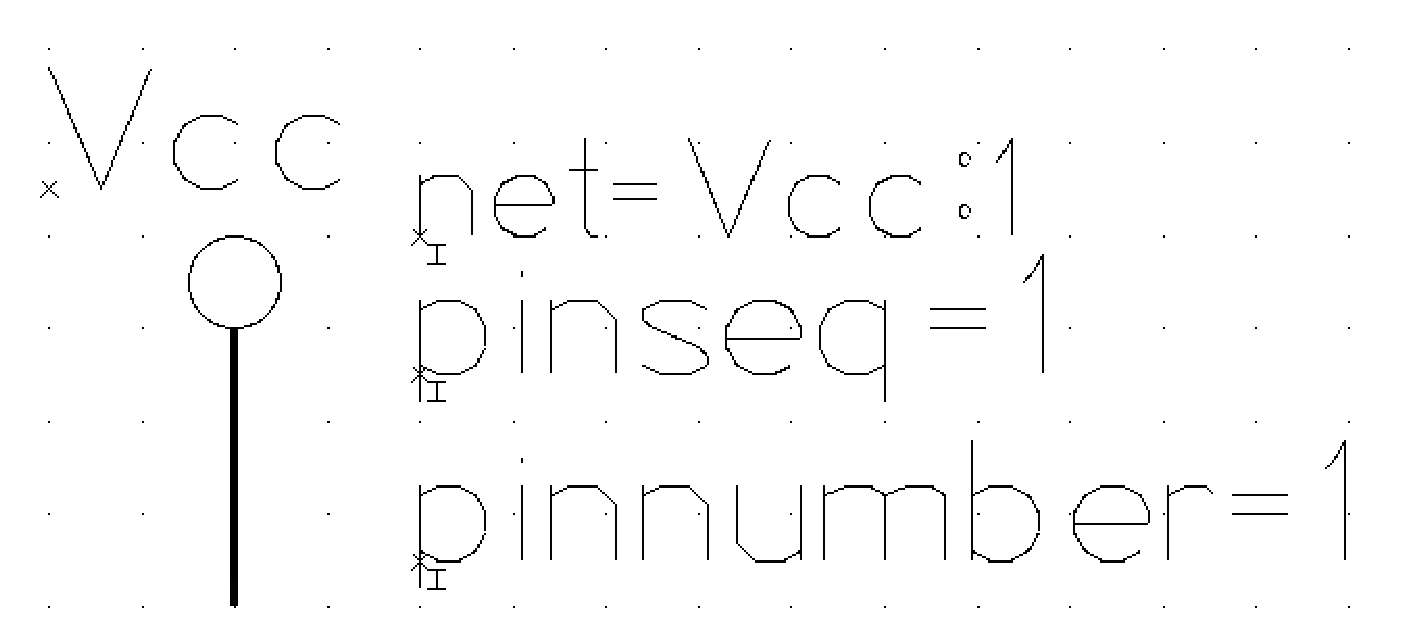
\includegraphics[clip,scale=0.2]{generic_vcc.eps}
		\caption{A power symbol with a hard-wired net attribute.  The attributes to the right of the symbol are made invisible on the schematic.\label{symbol_nonet}}
	\end{center} 
\end{figure}

\begin{figure}[ht]
	\begin{center}
		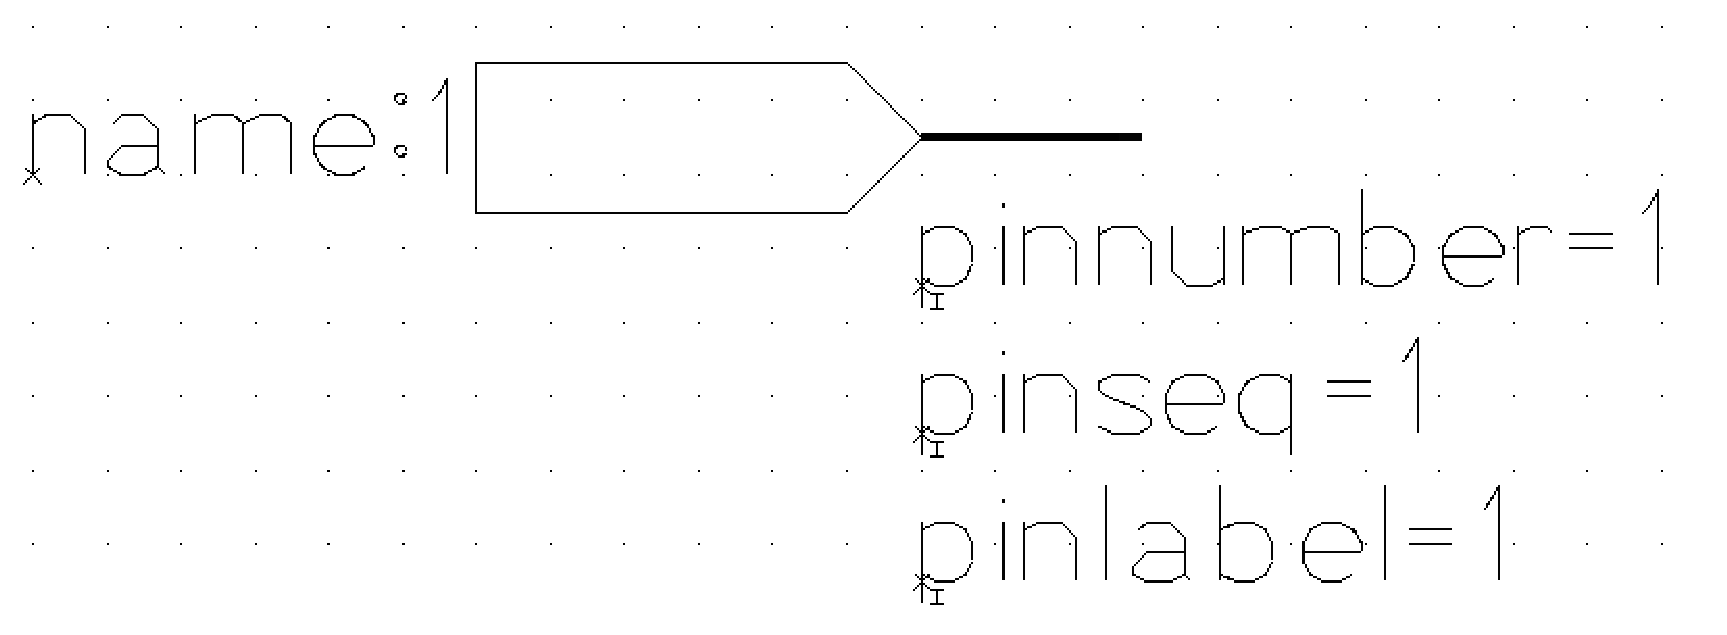
\includegraphics[clip,scale=0.2]{input_netname.eps}
		\caption{An off-page connector symbol with a net attribute you can change at the schematic level.  The attributes to the right of the symbol are made invisible on the schematic.\label{symbol_net}}
	\end{center} 
\end{figure}


\subsection{Changing attributes at the schematic level}
A part's default attributes can be overridden by editing the part within your schematic.  Selecting the part and clicking \textsl{Edit} $\rightarrow$ \textsl{Edit} (or using the \texttt{ee} shortcut) will bring up an ``Edit Attributes'' dialog box.  Here you can add new attributes to override the defaults.  For example, adding an attribute with the name ``footprint'' will override the footprint attribute taken from the symbol file.

%Miscellaneous notes
\subsection{General notes}
\begin{itemize}
	\item When you start gschem on a blank page, you'll be zoomed way out.  Zoom in a lot until the lines you draw snap to your visible grid.
	\item Multi-part devices should have a separate symbol for each part, named like part-a, part-b, etc.  For example, a single op-amp should have two symbols: one for the amplifier and one for its power pins.  Only the first device needs to have all the attributes -- the following devices only need reference designators.
	\item Op-amp symbols should be 0.8 inches high by 0.6 inches long.
	\item If a new device has the same symbol as one you've already drawn, just edit the text file and save it as a new part.
	\item Canned symbols are in \texttt{/usr/share/gEDA/sym}
	\item No line feeds are allowed in symbol files
	\item Part attributes must be associated with text -- you can't have a name=attribute entry in a symbol file without also having a text formatting line immediately above it.  This means that the pinnumber, pinseq, and pinlabel attributes will pile up on the schematic page if you make them visible.
\end{itemize}



